\subsubsubsubsection{StreetBuilder}
\begin{figure}[h]
\centering
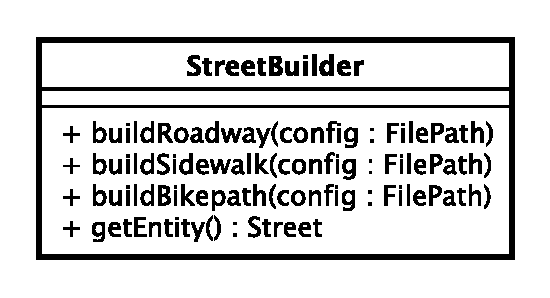
\includegraphics[scale=0.6,keepaspectratio]{images/solution/street_builder.eps}
\caption{App::Reactive::StreetBuilder}
\label{fig:sd-app-street_builder}
\end{figure}
\FloatBarrier
\begin{itemize}
  \item \textbf{Description} \\
    It represents the builder of street entities. 
  \item \textbf{Operation}
  \begin{itemize} 
    \item \texttt{+ buildTrafficLight()} \\
Adds a new traffic light to the street.
    \item \texttt{+ buildQueue()} \\
Adds a new queue of moving entities to the street.
    \item \texttt{+ getEntity() : Street} \\
Returns the street.
  \end{itemize}
\end{itemize}
